%!TEX root = user.tex
\chapter{Symbolic}
\label{CHAP: Symbolic}
\section{Introduction}
The \SYMBOL class in escript is used to define symbolic objects. The class extends Sympy\cite{Sympy}, a Python library for symbolic mathematics. The key 
addition in escript is the support for escript objects. \SYMBOL objects act as place holders for a single mathematical symbol, 
such as x, or for arbitrarily complex mathematical expressions such as
c * x**4 + alpha * exp(x) - 2 * sin(beta * x), where alpha, beta, c, and x
are also Symbols (the symbolic atoms of the expression).
With the help of the \EVALUATOR class these symbols and expressions can
be resolved by substituting numeric values and/or escript \Data objects
for the atoms. To facilitate the use of \Data objects, a \SYMBOL has a
shape (and thus a rank) as well as a dimension.
Symbols are useful to perform mathematical simplifications,
compute derivatives, take gradients and in the case of escript describe PDE's. As an example of how the symbolic toolbox can be used, consider the following code extract.
\begin{python}
import esys.escript as es
u = es.Symbol('u')
p = 2*u**2+3*u+1
p2 = es.sin(u)
p3 = p.diff(u)
evalu = es.Evaluator()
evalu.addExpression(p)
evalu.addExpression(p2)
evalu.addExpression(p3)
evalu.subs(u=2*es.symconstants.pi)
evaluated=evalu.evaluate()
print evaluated
\end{python}
Running this code evaluates to (1 + 6*pi + 8*pi**2, 0, 3 + 8*pi).  To get the answer evaluated we replace evalu.evaluate() with evalu.evaluate(evalf=True) this results in (98.8063911302536, 0, 28.1327412287183). This shows how the Symbols can be put into expressions and evaluated. The diff member used on p takes the derivative of p with respect to u. The use of these Symbols becomes more interesting in the context of escript when they are integrated with escript objects such as the \Data Object. 
\section{NonlinearPDE}
The NonlinearPDE class in escript has been implemented using interaction between escript symbols and escript objects such as domains. The NonlinearPDE class allows for the solution of PDEs of the form:
\begin{equation}
-div(X) + Y = 0
\label{symbolic eq1}
\end{equation}
where $X$ and $Y$ are function of $grad(u)$ and $u$ (the unknown function implemented as a \SYMBOL).
The intention is that X can be defined as an arbitrary function of the unknown function $u$ or $grad(u)$ to implement a desired equation.
The NonlinearPDE class uses the Symbolic class to solve the nonlinear PDE given in \eqn{symbolic eq1}
The class works by using Newton's method to find the zeroes of the left hand side of \eqn{symbolic eq1} and as a consequence finding the
$X$ and $Y$ which satisfy \eqn{symbolic eq1}. 
Newton's method involves evaluating the gradient of the function at $u_n$ and letting it go to 0 to get a $u_n$ from $u_{n-1}$. Consecutive updates are calculated until the equation is
satisfied to the desired level of accuracy. The solution to each update step involves solving a linear PDE. The NonlinearPDE class uses $X$ and $Y$ to produce the coefficient of the linear PDE for the update step. The linear PDE class given in \Sec{SEC LinearPDE} is used to solve the linear PDEs from the update step. The coefficients of the linear PDE to be solved are calculated as follows: \\\\
{
\centering 
 A = $\frac{\partial \text{X}}{\partial grad(u)}$   B = $\frac{\partial \text{X}}{\partial u}$   C = $\frac{\partial \text{Y}}{\partial grad(u)}$    D = $\frac{\partial \text{Y}}{\partial u}$
}
\section{2D Plane Strain Problem}
The NonLinearPDE class can be used to solve a 2D plane strain problem. In continuous media, stress is given by Lame's equation, \eqn{symbolic eq2}.
\begin{equation} 
-div(\sigma)=f
\label{symbolic eq2}
\end{equation} 
Hook's Law provides a relation between $\sigma$ and $\epsilon$ in the following form
\begin{equation}
\left[ \begin{array}{c}
\sigma_{00} \\
\sigma_{11} \\
\sigma_{01} \\
\end{array} \right] = 
\left[ \begin{array}{ccc}
c_{00} & c_{01} & c_{05}\\
c_{01} & c_{11} & c_{15}\\
c_{05} & c_{15} & c_{55}\\
\end{array}\right]
\left[ \begin{array}{c}
\epsilon_{00} \\
\epsilon_{11} \\
2\epsilon_{10} \\
\end{array} \right]
\label{symbolic eq3}
\end{equation}
Where $\epsilon = symmetric(grad(u)) \text{ or } \epsilon_{ij}=\frac{1}{2}\left(\frac{\partial u_i}{\partial x_j} + {\frac{\partial u_j}{\partial x_i}}\right)$ and 
u is the unknown function. To fit this to the nonlinear PDE class' standard form, X, is set to $c \times Symmetric(\text{grad(}u)))$ where $c$ is the stiffness matrix from \eqn{symbolic eq3}
The following python extracts show how an example 2D plane strain problem can be set up. 


\begin{python}
from esys.escript import *
from esys.finley import Rectangle
#set up domain and symbols
mydomain = Rectangle(l0=1.,l1=1.,n0=10, n1=10)
u = Symbol('u',(2,), dim=2)
q = Symbol('q', (2,2)
sigma = Symbol('sigma',(2,2))
theta = Symbol('theta')
# q is a rotation matrix represented by a Symbol. Values can be substituted for 
# theta.
q[0,0]=cos(theta)
q[0,1]=-sin(theta)
q[1,0]=sin(theta)
q[1,1]=cos(theta)
# Theta gets substituted by pi/4 and masked to lie between .3 and .7 in the 
# vertical direction. Using this masking means that when q is used it will apply
# only to the specified area of the domain. 
x = Function(mydomain).getX()
q=q.subs(theta,(symconstants.pi/4)*whereNonNegative(x[1]-.30)*whereNegative(x[1]-.70))
# epsilon is defined in terms of u and has the rotation applied. 
epsilon0 = symmetric(grad(u))
epsilon = matrixmult(matrixmult(q,epsilon0),q.transpose(1))
# For the purposes of demonstration, an arbitrary c with isotropic constraints 
# is chosen here. In order to act as an isotropic material c is chosen such that 
# c00 = c11 = c01+c1+2*c55
c00 = 10
c01 = 8; c11 = 10
c05 = 0; c15 = 0; c55 = 1
# sigma is defined in terms of epsilon
sigma[0,0] = c00*epsilon[0,0]+c01*epsilon[1,1]+c05*2*epsilon[1,0]
sigma[1,1] = c01*epsilon[0,0]+c11*epsilon[1,1]+c15*2*epsilon[1,0]
sigma[0,1] = c05*epsilon[0,0]+c15*epsilon[1,1]+c55*2*epsilon[1,0]
sigma[1,0] = sigma[0,1]
sigma0=matrixmult(matrixmult(q.transpose(1),sigma),q)
# set up boundary conditions
x=mydomain.getX()
gammaD=whereZero(x[1])*[1,1]
yconstraint = FunctionOnBoundary(mydomain).getX()[1]
# The nonlinear PDE is set up, the values are substituted in and the solution is
# calculated, y represents an external shearing force acting on the domain. 
# In this case a force of magnitude 50 is acting in the x[0] direction.
p = NonlinearPDE(mydomain, u, debug=NonlinearPDE.DEBUG0)
p.setValue(X=sigma0,q=gammaD,y=[-50,0]*whereZero(yconstraint-1),r=[1,1])
v = p.getSolution(u=[0,0])
\end{python}
%\pagebreak
The way in which the rotation matrix q is set up demonstrates the seamless integration of escript symbols and \Data objects. A \SYMBOL is used to set up the matrix, the values for theta are then later substituted in. The example also demonstrates how the symbolic toolbox can be used as an aid to easily move from a mathematical equation to an escript data object which can be used to do numerical calculations. 
Running the script calculates the unknown function u and assigns it to v. We can use v to calculate the stress and strain.  
\begin{table}[!h]
\centering
\begin{tabular}{|c|c|c|}
  \hline
   & Anisotropic & Isotropic\\%\multicolumn{2}{|c|}{Isotopic} \\
  \hline
  No rotation & 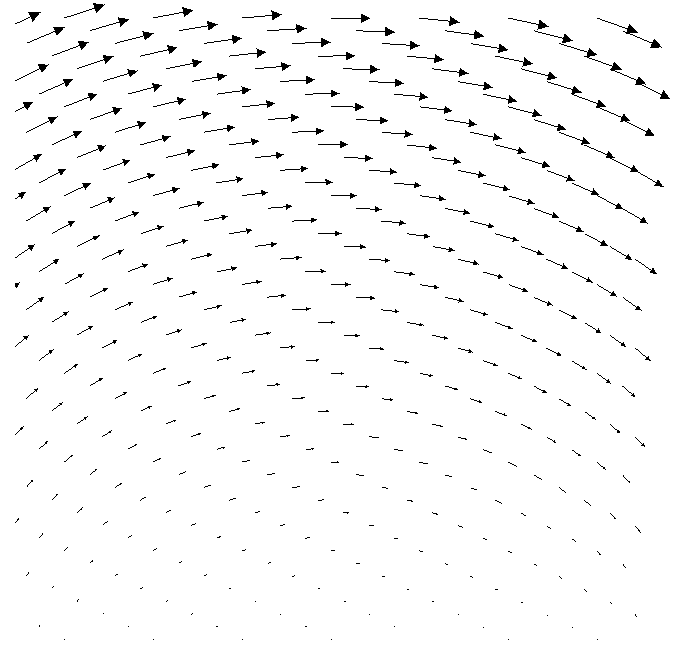
\includegraphics[scale=0.2]{0RotAniso} & 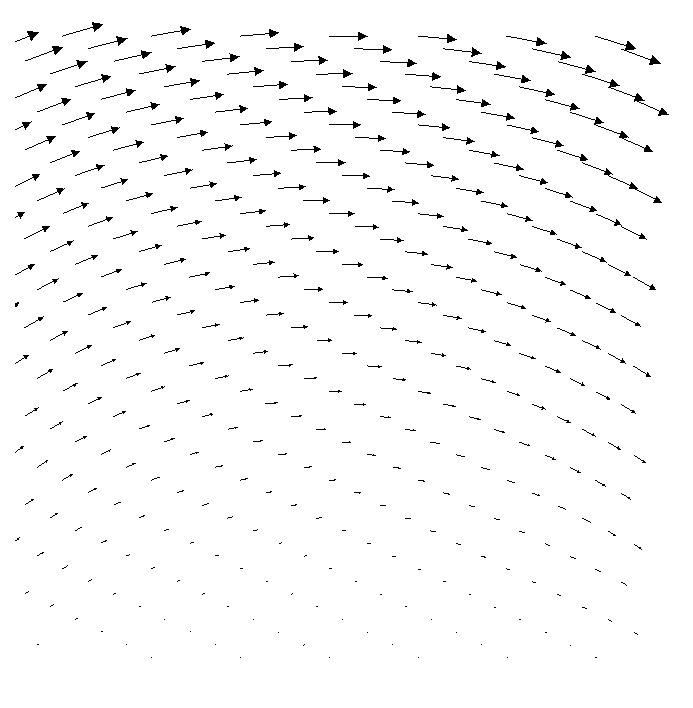
\includegraphics[scale=0.2]{0RotIso}\\
  \hline
  60\textdegree rotation & 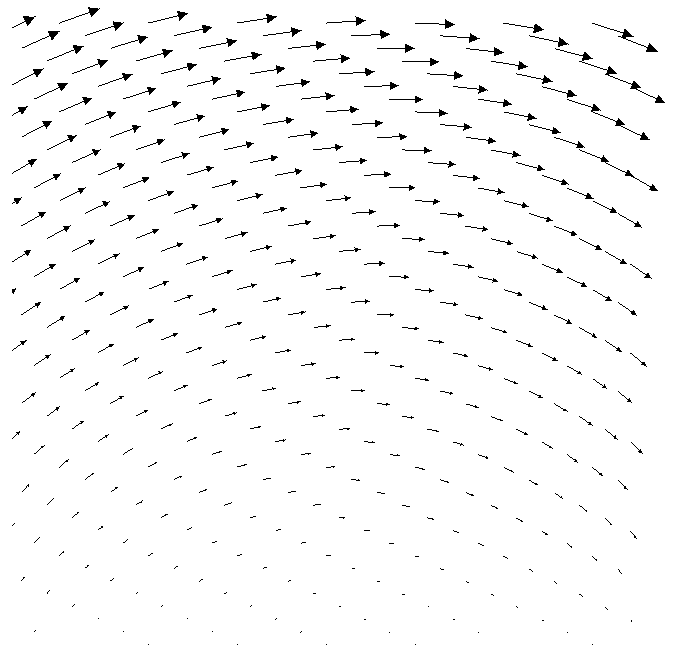
\includegraphics[scale=0.2]{MidRotAniso} & 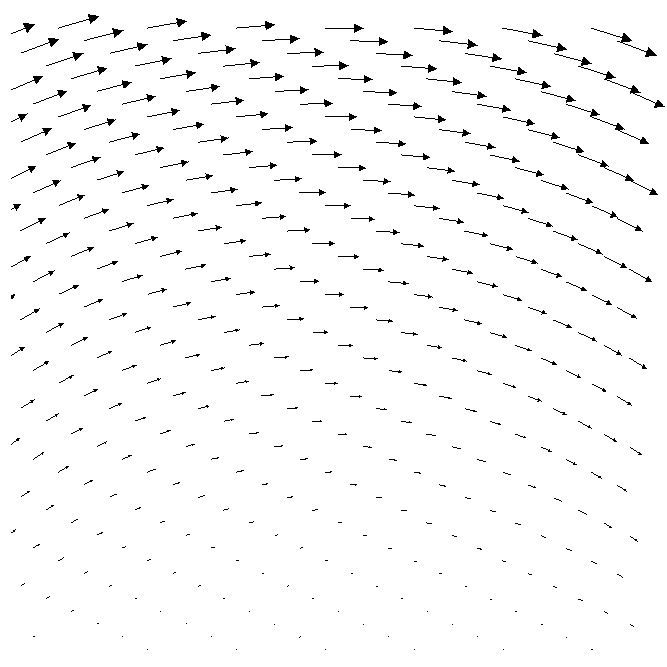
\includegraphics[scale=0.2]{MidRotIso}\\ 
  \hline
  difference & 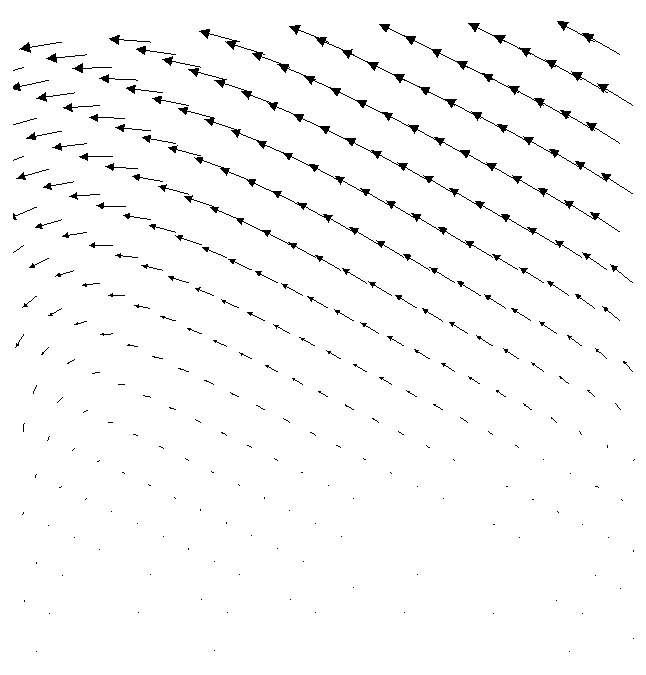
\includegraphics[scale=0.2]{diffaniso} & 
\includegraphics[scale=0.2]{diffiso}\\ 
  \hline
\end{tabular}
\caption{Displacement vectors calculated using NonlinearPDE}
\label{isovsaniso}
\end{table}
Table \ref{isovsaniso}, shows the result of running the above script under varying values of c and theta. Both an isotropic and ansisotropic case are considered.  For the anisotropic case, c is chosen such that c00 = c11 = c01+c1+2*c55 does not hold. Two cases of theta are also considered; one with a masked 60\textdegree rotation in the middle and one with no rotation. The last row of the table shows the difference between rotation in the middle and no rotation. In the isotropic case it can be seen that there is no difference in the output when the rotation is applied. There is however an obvious difference when the anisotropic case is considered.   

\newpage
\section{Classes}
A number of classes are associated with escript symbols. A detailed listing of the definitions and usage is provided below. 
\subsection{Symbol class}
\begin{classdesc}{Symbol}{symbol \optional{, shape} \optional{, Dim}}
Defines a \SYMBOL object. The first argument \SYMBOL is a string given to represent the \SYMBOL. The string typically matches the name of the object, for instance u=Symbol('u'). Next the shape defines whether the \SYMBOL is a vector or a matrix etc up to a 4 tensor and the length or size of it. Dim is used to define the dimensionality of the object contained in the \SYMBOL.
For a \SYMBOL definition u = Symbol('u',(10,), dim=2), u will be a 10 component vector of 2 dimensional objects.
\end{classdesc}
\subsubsection{Symbol class methods}
\begin{methoddesc}[Symbol]{atoms}{\optional{types}}
Returns the atoms that form the current \SYMBOL.
By default, only objects that are truly atomic and cannot be divided
into smaller pieces are returned: symbols, numbers, and number
symbols like I and pi. It is possible to request atoms of any type,
however.
\end{methoddesc}

\begin{methoddesc}[Symbol]{coeff}{x \optional{, expan=true}}
Returns the coefficient of the term x or 0 if there is no x.
If x is a scalar \SYMBOL then x is searched in all components of
this \SYMBOL. Otherwise the shapes must match and the coefficients are
checked component by component.
Example:
\begin{python}
     x=Symbol('x', (2,2))
     y=3*x
     print y.coeff(x)
     print y.coeff(x[1,1])
\end{python}
will print:
\begin{python}
     [[3 3]
      [3 3]]
     [[0 0]
      [0 3]]
\end{python} 
\end{methoddesc}
\begin{methoddesc}[Symbol]{diff}{symbols}
Takes the derivative of the symbol object which the method belongs to with respect to the symbols specified in the argument symbols.
\end{methoddesc}
\begin{methoddesc}[Symbol]{evalf}{}
Applies the sympy.evalf operation on all elements of the \SYMBOL which are of type or inherit from sympy.Basic 
\end{methoddesc}
\begin{methoddesc}[Symbol]{expand}{}
Applies the sympy.expand operation on all elements in this \SYMBOL.
\end{methoddesc}
%\begin{methoddesc}[Symbol]{getDataSubstitutions}{}
%end{methoddesc}
\begin{methoddesc}[Symbol]{getDim}{}
Returns the symbol's spatial dimensionality, or -1 if undefined
\end{methoddesc}
\begin{methoddesc}[Symbol]{getRank}{}
Returns the symbol's rank which is equal to the length of the shape.
\end{methoddesc}
\begin{methoddesc}[Symbol]{getShape}{}
Returns the shape of this \SYMBOL.
\end{methoddesc}
\pagebreak
\begin{methoddesc}[Symbol]{grad}{\optional{where=none}}
Returns the gradient of the \SYMBOL to which the function is applied. The \SYMBOL must have a dimensionality defined in order for grad to work. As with the normal escript grad a \FunctionSpace can be specified using the where argument. The \FunctionSpace should be wrapped in a \SYMBOL. To do this, set up a \SYMBOL and then use the 'subs' function to substitute in the \FunctionSpace.
\end{methoddesc}
\begin{methoddesc}[Symbol]{inverse}{}
Find the inverse of the \SYMBOL to which the function is applied. Inverse is only valid for square rank 2 symbols.
\end{methoddesc}
%\begin{methoddesc}[Symbol]{item}{}
%\end{methoddesc} 
%\begin{methoddesc}[Symbol]{lambdarepr}{}
%test
%\end{methoddesc}
\begin{methoddesc}[Symbol]{simplify}{}
Applies the sympy.simplify operation on all elements in this \SYMBOL.
\end{methoddesc}
\begin{methoddesc}[Symbol]{subs}{old,new}
Substitutes or replaces a \SYMBOL specified in old with whatever is in new for the \SYMBOL which it is called on. Consider:
  \begin{python}
     import esys.escript as es
     u=es.Symbol("u")
     expr=2*u
     expr.subs(u,2)
\end{python}
This prints 4.
\end{methoddesc}
\begin{methoddesc}[Symbol]{trace}{axis_offset}
Returns the trace of the \SYMBOL object.
\end{methoddesc}


\subsection{Evaluator class}
The \EVALUATOR class is intended to have a group of expressions added to it, substitutions can be made across all expressions and the expressions can then all be evaluated.
\subsubsection{Evaluator class methods}
\begin{classdesc}{Evaluator}{\optional{expressions}}
An \EVALUATOR object is initiated via Evaluator() with an optional argument of expressions to store.
\end{classdesc}
\begin{methoddesc}[Evaluator]{addExpression}{expression}
Adds an expression to this \EVALUATOR.
\end{methoddesc}
\begin{methoddesc}[Evaluator]{evaluate}{\optional{evalf=False}\optional{, args}}
Evaluates all expressions in this \EVALUATOR and returns the result as a tuple.  Evalf can be set to true to call evalf on any sympy symbols which may be part of the expression.
Args can be provided to make any substitutions before the expression is evaluated.
\end{methoddesc}
\begin{methoddesc}[Evaluator]{subs}{old,new}
Substitutes or replaces a \SYMBOL specified in old with whatever is in new for all expressions in the \EVALUATOR.
\end{methoddesc}

\subsection{NonlinearPDE class}
\begin{classdesc}{NonlinearPDE}{domain, u}
Defines a general nonlinear, steady, second order PDE for an unknown function \var{u} on a given domain defined through a \Domain object \var{domain}. \var(u) is a \SYMBOL object.
The general form is -div(X) + Y = 0 
\end{classdesc}
\iffalse
\begin{methoddesc}[NonlinearPDE]{concatenateRow}{}
test
\end{methoddesc}
\begin{methoddesc}[NonlinearPDE]{createCoefficient}{}
test
\end{methoddesc}
\begin{methoddesc}[NonlinearPDE]{getUnknownSymbol}{}
test
\end{methoddesc}
\begin{methoddesc}[NonlinearPDE]{getLinearSolverOptions}{}
test
\end{methoddesc}
\begin{methoddesc}[NonlinearPDE]{getLinearPDE}{}
test
\end{methoddesc}
\begin{methoddesc}[NonlinearPDE]{getNumSolutions}{}
test
\end{methoddesc}
\begin{methoddesc}[NonlinearPDE]{getShapeOfCoefficient}{}
test
\end{methoddesc}
\begin{methoddesc}[NonlinearPDE]{getCoefficient}{}
test
\end{methoddesc}
\begin{methoddesc}[NonlinearPDE]{getSensitivity}{}
test
\end{methoddesc}
\fi
\begin{methoddesc}[NonlinearPDE]{getSolution}{subs}
Returns the solution of the PDE. Substitutions for all symbols used in the coefficients including the initial value for the unknown u.
\end{methoddesc}
\pagebreak
\begin{methoddesc}[NonlinearPDE]{setOptions}{opts}
\begin{verbatim}
Allows setting options for the nonlinear PDE.
The supported options are:
  tolerance
      error tolerance for the Newton method
  iteration_steps_max
      maximum number of Newton iterations
  omega_min
      minimum relaxation factor
  atol
      solution norms less than atol are assumed to be atol.
      This can be useful if one of your solutions is expected to
      be zero.
  quadratic_convergence_limit
      if the norm of the Newton-Raphson correction is reduced by
      less than quadratic_convergence_limit between two iteration
      steps, quadratic convergence is assumed.
  simplified_newton_limit
      if the norm of the defect is reduced by less than
      simplified_newton_limit between two iteration steps and
      quadratic convergence is detected, the iteration switches to the
      simplified Newton-Raphson scheme.
\end{verbatim}

\end{methoddesc}
\begin{methoddesc}[NonlinearPDE]{setValue}{
\optional{X}\optional{, Y}
\optional{, d}\optional{, y}
\optional{, d_contact}\optional{, y_contact}
\optional{, q}\optional{, r}}
Assigns new values to coefficients. By default all values are assumed to be
zero\footnote{In fact, it is assumed they are not present by assigning the
value \code{escript.Data()}. This can be used by the solver library to reduce
computational costs.}.
If the new coefficient value is not a \Data object, it is converted into a
\Data object in the appropriate \FunctionSpace.
\end{methoddesc}

\subsection{Symconsts class}
Symconsts provides symbolic constants for use in symbolic expressions. These constants are preferred to floating point implementation as they can cancel perfectly when mathematical expressions are evaluated, avoiding numerical imprecision. 
\begin{verbatim}
usage:
  symconsts.pi this provides a \SYMBOL object
  
Available constants currently include:
  pi and e 
\end{verbatim}


